% CS213 Assignment 2
% Introduction to Beamer
% Submitted by:
% Omkar D Jadhav,
% 190010029, CSE

\documentclass{beamer}
\usepackage[utf8]{inputenc}
\usepackage{graphicx}
\usepackage{blindtext}
\usetheme{Madrid}
\usecolortheme{default}
\usepackage{amsfonts}
\usepackage{hyperref}
\usepackage{multirow}
\usepackage{amsmath} 
\title{CS213 Assignment 2}
\subtitle{Introduction to Beamer}
\setbeamerfont{institute}{size=\small}
\author{Omkar D Jadhav}
\institute[IIT Dharwad]{\linespread{1.3}Department of Computer Science and Engineering \\ IIT Dharwad
      \\ Email: \texttt{190010029@iitdh.ac.in}}  %Using alternate institute name for footer
\date{September 2020}
\logo{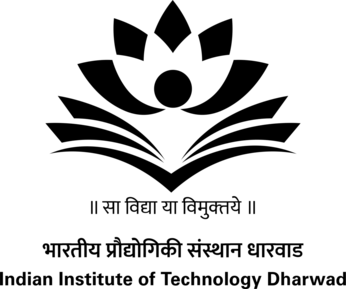
\includegraphics[height=1.5cm]{logo.png}}
\setbeamertemplate{theorems}[numbered]
\begin{document}

\frame{\titlepage}  % building titlepage using given info above
\section{Introduction}
\begin{frame}
\label{overlay1}
\frametitle{Usage of Overlays}
\framesubtitle{Stepwise viewing}
A. Using pause method on lists:
\begin{itemize}
    \item This section uses pause method to view content stepwise 
    \pause                                                              %using \pause to stop flow
    \item Presentor is supposed to click a button to move to next content.
    \pause
    \item It could be used for any sort of content like figures,lists etc.
    \pause
    \item Next slide will use pause method on figures and blocks.
    
\end{itemize}
\end{frame}

\begin{frame}[t]
\frametitle{Usage of Overlays}
\framesubtitle{Stepwise viewing}
\transblindshorizontal
{B. Using pause method on figures and blocks: \pause
\begin{columns}
\begin{column}{0.48\textwidth}
\centering

\includegraphics[height=3cm]{overleaf.png} \pause
\end{column}
\begin{column}{0.48\textwidth}
\centering

\includegraphics[height=3cm]{sharelatex.png} \pause
\end{column}
\end{columns}

\begin{block}{Dummy block}
This is a dummy block.
\end{block}
\pause
\begin{columns}
\begin{column}{0.7\textwidth}
\begin{alertblock}{Alert block}
This is an alert block.
\end{alertblock}
\end{column}
\end{columns}
}
\end{frame}

\begin{frame}
\frametitle{Usage of Overlays}
\framesubtitle{Stepwise viewing}
C. Using onslide method for text. \pause \\ \vfill
\setbeamercovered{transparent}
\onslide<2->{This section is meant to show usage of onslide} \\
\onslide<3-5>{I will disappear after next 2 slides} \\
\onslide<4->{I will stay till the end} \\
\onslide<5-5>{I will disappear right after this slide} \\
\onslide<6->{I will stay till the end}\\
\onslide<7->{The end}\\
\end{frame}

\begin{frame}[t]
\frametitle{Usage of Overlays}
\framesubtitle{Stepwise viewing}
\transblindsvertical{
C. Using onslide method on figures and blocks: \pause
\begin{columns}
\begin{column}{0.48\textwidth}
\centering
\onslide<2->{

\includegraphics[height=3cm]{overleaf.png} }
\end{column}
\begin{column}{0.48\textwidth}
\centering
\onslide<3->{

\includegraphics[height=3cm]{sharelatex.png}}
\end{column}
\end{columns}

\onslide<4-4>{ \begin{block}{Dummy block}
This is a dummy block. I will disappear next.
\end{block} }

\begin{columns}
\begin{column}{0.7\textwidth}
\onslide<5->{
\begin{alertblock}{Alert block}  % block with default red colour
This is an alert block.
\end{alertblock}}
\end{column}
\end{columns}
}
\end{frame}


\begin{frame}[t]
\label{overlay2}
\frametitle{Usage of Overlays}
\framesubtitle{Replace commands }
\textbf{A. Using only command:}\\ \pause
\only<2>{ Hello, only command has been applied to me.}
\only<3>{ I am similar to visible command but I don't take up additional space}
\only<4>{ For example: \textit{ \blindtext}}
\only<5>{ Next commands to be explored are visible and invisible commands:}
\onslide<6->{Done.} \\
\onslide<6->{\textbf{B. Using visible and invisible command}} \\
\visible<7-7>{Hello, visible command has been applied to me. I will be invisible after 1 skip}\\
\visible<8->{As you can see, previous text disappeared but it still takes up the space given to it.} \\
\visible<9->{\centering In this way,visible is different than only.}\\
\visible<10->{\centering In the next slide we will see the Usage of Highlighting.}\\

\end{frame}

\begin{frame}
\label{overlay3}
\frametitle{Usage of Overlays}
\framesubtitle{Highlighting commands }
\begin{itemize}
\item The command alert has been applied to the word \alert{Highlighted} .\pause \\
\item We can also use normal color command to {\color<3->{blue}{highlight}}.\pause\\
\item This way we can customise alerts with any colours, be it {\color<4->{blue}{Blue}}, {\color<5->{green}{Green}} or any colour. \\
\end{itemize}

\begin{alertblock}{Alert!}
Sometimes alertblock is used instead of alert command.
\end{alertblock}

\end{frame}

\begin{frame}[t]
\frametitle{Usage of Hyperlinks}
\transboxout{
\begin{itemize}
    \item \textbf{In this slide we see inclusion of hyperlinks}
    \item  This \alert{\href{www.iitdh.ac.in}{link}} leads to IIT Dharwad website.\\
    \item We could also use url command if no url description is needed.
    \item \url{www.iitdh.ac.in}
    \item Hyperlinks can be used to go to different slides like following.

\end{itemize}
{\centering
\hyperlink{overlay1}{\beamergotobutton{Stepwise viewing}}\\
\hyperlink{overlay2}{\beamergotobutton{Replace commands}}\\
\hyperlink{overlay3}{\beamergotobutton{Highlight commands}}\\
}
}
\end{frame}

\begin{frame}[t]
\label{imguse}
\frametitle{Usage of Structures}
\framesubtitle{Columns and blocks}
 \textbf{In this slide we see usage of columns and blocks}
 
 \begin{columns}
    \begin{column}{0.4\textwidth}
        \begin{itemize}
    \item  This is the first of the three columns present
    \item Any column can contain any sort of content.
    \item 2nd column contains blocks.
    \item 3rd column contains an image.

    \end{itemize}
    \end{column}
    \begin{column}{0.35\textwidth}
        \begin{block}{Block}
        This is a sample block inside a column.
        \end{block}
        \begin{alertblock}{Alert Block}
        This is an alert block inside a column.
        \end{alertblock}
    \end{column}
    \begin{column}{0.25\textwidth}
    \centering
    \begin{figure}
        \centering
        
\includegraphics[height=2cm]{overleaf.png}
    \end{figure}
    \end{column}
\end{columns}
\vfill
{
Further slides include concepts which have been covered already \\ in \LaTeX\ assignment.}

\end{frame}

\begin{frame}[t]
\frametitle{Figures and Tables}
\transglitter{
\textbf{Figures:} Figures have been used throughout the document. For example \alert{\hyperlink{imguse}{this slide.}}\\
\textbf{Tables:} Following are some tables with multirows and multicolumns. \ \vfill \pause

\centering
\begin{tabular}{|c|c|c|c|}
\hline
     & \multicolumn{3}{|c|}{Countries}\\
     \cline{2-4}
Year & India & Afghanistan & Bangladesh \\ 
\hline
2000 & 1.8 & 1.9 & 1.4 \\
2005 & 1.5 & 1.9 & 1.4 \\
2006 & 1.4 & 2.0 & 1.3 \\
2007 & 1.5 & 2.0 & 1.3 \\
2008 & 1.4 & 2.0 & 1.3  \\
2009 & 1.4 & 2.0 & 1.3 \\
\hline
      
\end{tabular}

}

\end{frame}

\begin{frame}[t]
\frametitle{Continuation of tables, Transitions}
\transwipe{
\centering
\begin{tabular}{|c|c|c|c|c|} %vertical lines 
\hline
\multicolumn{3}{|c|}{\multirow{2}{*}{Nested multicol-multirow}}& A & B \\ 
\cline{4-5}
\multicolumn{3}{|c|}{}&C&D\\
\hline
E&F&\multicolumn{3}{|c|}{multicol}\\
\hline
\multicolumn{5}{|c|}{G}\\  
\hline
\end{tabular}
\\
\vfill
\textbf{Transitions: }
Many of the slides have transitions attached to them.\\
\vfill
In the next slide we have Mathematics section.
}
\end{frame}

\begin{frame}[t]
\frametitle{Mathematics section}

\begin{theorem}
 If $q^2 $ is divisible by $3$, so is $q$.
 \end{theorem}
 \begin{theorem}
 $ \sqrt{3} $ is irrational.
 \end{theorem}
\begin{proof}
    Suppose not;  i.e.,  suppose $\sqrt{3} \in \mathbb{Q}$. Then $\exists$ m,n $\in \mathbb{Z}$ with m and n relatively prime and $\sqrt{3} = \frac{m}{n}$. Then $3n^2=m^2$.Thus $m^2$ is divisible by 3 so by Theorem 1 ,m is also.\\ \pause By definition,m = 3k for some k $\in \mathbb{Z}.$  Hence $m^2= 9k^2= 3n^2$ and so $3k^2 = n^2.$ Thus $n^2$ is divisible by 3 and again by Theorem 1,n is also divisible by 3.  But m,n are relatively prime, a contradiction. Thus $\sqrt{3} \notin \mathbb{Q}.$ 
\end{proof}
    
\end{frame}

\begin{frame}[t]
\frametitle{Mathematics section}
\textbf{Multiline equation (with step viewing)}\\
\begin{eqnarray*}
    \cos 2\theta & = \pause & \cos^2 \theta - \sin^2 \theta \\ \pause
                 & =  & 2\cos^2 \theta -1 \\ \pause
                 & =  & 1- 2\sin^2 \theta
\end{eqnarray*}
\vfill
\textbf{Next slide shows explicit use of lists with step viewing}\\

    
\end{frame}

\begin{frame}[t]
\frametitle{Lists}
\framesubtitle{Itemize, Enumerate, Description}
\begin{columns}
\begin{column}{0.5\textwidth}
\onslide<1->{\textbf{Itemize}} \\
\begin{itemize}
    \item<2-> This is the start of the list
    \item<3-> In this type of list items have bullet points with them.
    \item<4-> It is also called unordered list.
    \item<5-> This is the end of the list
\end{itemize}

\end{column}
\begin{column}{0.5\textwidth}
\onslide<1->{\textbf{Enumerate}}\\
\begin{enumerate}
    \item<2-> This is the start of the list
    \item<3-> In this type of list items have numbering with them.
    \item<4-> It is also called ordered list.
    \item<5-> This is the end of the list
\end{enumerate}
\end{column}
\end{columns}
\vfill
\onslide<1->{\textbf{Description}}\\
\centering
\begin{description}
    \item<2-> [First] 
    This is the start of the list
    \item<3-> [Second] 
    In this type of list items have title attached  with them.
    \item<4-> [Third]
    It is also called Descriptive list.
    \item<5-> [Fourth]
    This is the end of the list
\end{description}

\end{frame}

\begin{frame}
\begin{center}
\Huge Thank You!
\end{center}
\end{frame}

\end{document}
